\documentclass[12pt,DIV=14, version=first, BCOR=10mm,a4paper,twoside,parskip=half-,headsepline,headinclude]{scrartcl}
% Grundgröße 12pt, zweiseitig scrartcl
% Standardpakete
\usepackage[utf8]{inputenc}
\usepackage[T1]{fontenc}
\usepackage{lmodern}
% deutsche Silbentrennung
\usepackage[ngerman]{babel}
% schöne Tabellen
\usepackage{booktabs}
% etwas Mathematik
\usepackage{amsmath,amssymb}
% Grafiken einbinden
\usepackage{graphicx}
\usepackage{wrapfig}
% Kopf- und Fußzeilen
\usepackage[headsepline,footsepline,automark]{scrlayer-scrpage}
\pagestyle{scrheadings}
% Links anklickbar
\usepackage{url,hyperref,color} 
\definecolor{MidnightBlue}{cmyk}{0.98,0.13,0,0.43}
\hypersetup{colorlinks,breaklinks=true, pdffitwindow=true,pdfpagelayout=SinglePage,
            linkcolor=blue,pdfauthor={}, pdfdisplaydoctitle=true,
            pdfsubject={},   % to be defined later
            bookmarksnumbered,citecolor=MidnightBlue, 
            urlcolor=MidnightBlue}
\raggedbottom
\renewcommand{\topfraction}{1}
\renewcommand{\bottomfraction}{1}


% einbinden der Literatur     
\usepackage[T1]{fontenc}
\usepackage{babel}
\usepackage{csquotes}
\usepackage[
  backend=biber,
  style=numeric-verb,
  block=ragged,
  urldateusetime=true,
]{biblatex}
\addbibresource{refs.bib}


% jetzt gehts los
\begin{document}% hier gehts los
\thispagestyle{empty} % Titelseite

\includegraphics[width=0.2\textwidth]{hsh_logo/Wortmarke_WI_schwarz}

{~ \sffamily
    \vfill
    {\Huge\bfseries Die Grundlagen der Computer-Forensik}
    \bigskip

    {\Large 
    Schehat Abdel Kader und Detijon Lushaj \\[2ex]
    Seminar-Arbeit im Studiengang "`Angewandte Informatik"'
    \\[5ex]
    \today } 
}
\vfill
~ \hfill

\includegraphics[height=0.3\paperheight]{hsh_logo/H_WI_Pantone1665} 

\vspace*{-3cm}

\newpage \thispagestyle{empty}

\begin{tabular}{ll}
{\bfseries\sffamily Autor 1:}   & Schehat Abdel Kader (SAK)\\ 
                                & 1630110 \\
                                & schehat.abdel-kader@stud.hs-hannover.de \\[5ex]
{\bfseries\sffamily Autor 2:}   & Detijon Lushaj (DL)\\  
                                & 1630149 \\
                                & Detijon.lushaj@stud.hs-hannover.de \\[5ex]
 {\bfseries\sffamily Prüfer:}   & M. Sc. Frank Müller \\
          	                    & Abteilung Informatik, Fakultät IV \\
         	                    & Hochschule Hannover \\
        	                    & frank.mueller@hs-hannover.de
\end{tabular}

\vfill

\begin{center} \sffamily\bfseries Selbständigkeitserklärung \end{center}
% fett und zentriert in der minipage

Mit der Abgabe der Ausarbeitung erklären wir, dass wir die eingereichte Seminar-Arbeit
selbständig und ohne fremde Hilfe verfasst, andere als die von uns angegebenen Quellen
und Hilfsmittel nicht benutzt und die den benutzten Werken wörtlich oder
inhaltlich entnommenen Stellen als solche kenntlich gemacht haben. 
\vspace*{7ex}

Hannover, den \today \hfill 

\pagebreak
\pdfbookmark[0]{Inhalt}{contents}
\tableofcontents
\pagebreak

% durch eigenen Text ersetzen
\section {Einleitung DL}
In der Seminararbeit werden die Grundlagen der Computer-Forensik eingeführt und erläutert. Bietet eine kurze Einführung in die Methoden der Computer-Forensik und listet die Anforderungen an forensische Untersuchungen und Beweissicherung auf.

	\subsection {Motivation}
	Die heutige Welt wird von Computern dominiert. Auch die tägliche Nutzung von Computern in den unterschiedlichsten Branchen und kritischer Infrastrukturen erhöht das Missbrauchsrisiko. Die Zahl der Straftaten im Zusammenhang mit Computern hat in den letzten Jahrzehnten exponentiell zugenommen. Auch ein Bericht des Bundesamtes für Sicherheit in der Informationstechnik zeigt, wie in \autoref{fig:stat} dargestellt eine generelle Zunahme potenzieller Risiken \cite[vgl. S. 11]{BSI_lagebericht}.
	
	\begin{figure}[h] 
		% Die Option [h] sagt LaTeX, wo die Grafik im Text platziert werden soll. 
		% (h)ere, (t)op, (b)ottom oder die Platzierung auf der nächsten (p)age.
		\centering %mittig zentriert
		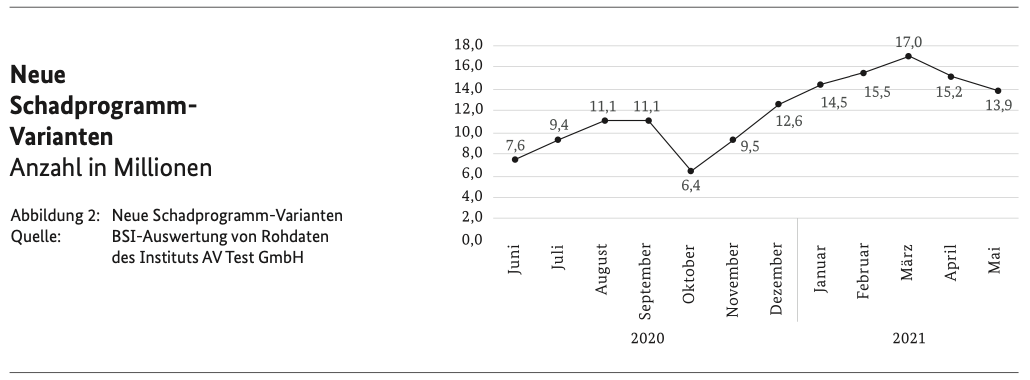
\includegraphics[width=1\textwidth]{bilder/stat_Schadprogramm.png} 
		\caption{Neue Schadprogramm-Variante 2021 des BSI \cite[S. 11]{BSI_lagebericht}} 
		\label{fig:stat}
	\end{figure}
	
	Bei diesen Straftaten handelt es sich hauptsächlich um Betrug und Vandalismus. Aufgrund der dramatischen Zunahme von Straftaten wächst auch das Interesse an Methoden zur Strafverfolgung oder Ermittlung von Tätern, Schadensersatz und Prävention dieser Straftaten.
	
	\subsection{Ziel der Arbeit}
	In dieser Seminararbeit werden die verschiedenen Aspekte der Computer-Forensik dargestellt. Zunächst werden Vorüberlegungen über die Bedrohungssituation getroffen. Anschließend die Anforderungen an den Ermittlungsprozess gestellt und die Grundlagen der Computer-Forensik beschrieben. Abschließend, welche Daten wie aufgezeichnet werden müssen, sodass diese juristisch belastbar sind und Auskunft über die ersten Schritte nach einem Vorfall.
	
	\subsection {Begriffserklärung Computer-Forensik}
	Der Begriff Computer-Forensik bezeichnet die Analyse und Aufklärung von Sicherheitsvorfällen. Ermittler und Ermittlerinnen suchen wie in anderen Bereichen der Forensik nach digitalen Spuren, die Hinweise auf Verbrechen liefern sollen. Typische Beispiele sind Hackerangriffe oder Datenschutzverletzungen durch Insider. Computerforensische Untersuchungen werden immer unmittelbar nach einer Straftat oder einem Verdachtsfall durchgeführt.

	\subsection{Ziele}
	Der Zweck einer forensischen Untersuchung besteht darin, Beweise zu liefern, um die Hypothese zu stützen, dass das System kompromittiert wurde. In diesem Fall führt ein Expertenteam eine forensische Untersuchung durch, um aufzudecken, ob und wann ein System angegriffen wurde, wer die mutmaßlichen Angreifer und Angreiferinnen sind und welche Sicherheitslücken ausgenutzt werden konnten, um das System zu infiltrieren. Darüber hinaus soll die forensische Analyse das Ausmaß des Schadens ermitteln und Beweise zum Sicherheitsvorfall für weitere rechtliche Schritte sichern \cite[vgl. S. 65]{texbook01}. Die Schwierigkeit beim Erreichen dieser Ziele liegt darin, die richtigen Daten sicher zu sammeln, ohne den Zustand des kompromittierten Systems zu ändern.

\section{Bedrohungssituation DL}
\begin{quote}
    \glqq
    Mit Bedrohung ist der potenzielle Auslöser für ein unerwünschtes Ereignis gemeint, das sich auf das betroffene IT-System oder die gesamte Organisation schädlich auswirken kann. 
    \grqq
    \cite[S.11]{texbook01}
\end{quote}

Unternehmen und ihre IT-Umgebungen sind vielfältigen Bedrohungen ausgesetzt.
Grundsätzlich wird angestrebt diese Bedrohungen abzuwehren, allerdings ist das häufig nicht möglich. Sicherheitsverantwortliche müssen diese Bedrohungen identifizieren und ihren Schweregrad und ihre Eintrittswahrscheinlichkeit bewerten. Zudem spielt die Frage der Herkunft und die Motivation des potenziellen Täters eine wichtige Rolle.


    \subsection{Risikoverteilung}
    Um ein Risiko angemessen einzustufen, ist dessen Wahrscheinlichkeit für eine Gefährdung durch ein solches Ereignis und das zu erwartende resultierende Schadensausmaß zu beurteilen. Die Eintrittswahrscheinlichkeit und Schadenshöhe sind somit die maßgeblichen Parameter, um das eigene Risiko einzuschätzen \cite[vgl. S. 12]{texbook01}.
    Aus diesem Grund ist es zugunsten eines Unternehmens herauszufinden, welche Unternehmenswerte gefährdet sein können. Dazu zählen auch Betrachtungen, wie weit der Schaden an den Unternehmenswerten und dem Unternehmen insgesamt im Falle einer Kompromittierung reicht, wie hoch die Wahrscheinlichkeit eines Schadens ist und wo es noch vorhandene Schwachstellen gilt auszubessern.
    Aufgrund dieser aufgeführten Erkenntnisse bietet es sich in den meisten Fällen an, Sicherheitsmaßnahmen auf organisatorischer, technischer und auch personeller sowie infrastruktureller Ebene umzusetzen.

    Bezüglich der Zunahme der Zahl angegriffener Systeme ist ein Zusammenhang mit der Zahl vernetzter Computersysteme zu erkennen. Ein Grund, der in diesem Zusammenhang beisteuert, ist eine erhöhte Anzahl an potenziellen Zielen, die durch das Vernetzen ermöglicht werden \cite[vgl. S. 13]{texbook01}.
    Hierbei reicht das Vernetzen über das Internet von mehreren Systemen aus, um für das Aufkommen neuer krimineller Gruppen mit vielfältigen Motiven zu sorgen.
    Ebenfalls ist zu beobachten, dass die Angriffstechniken immer komplexer werden und das Hauptproblem dabei in der Zugänglichkeit und den erleichterten Anforderungen in der Bedienung solcher Tools liegt.

    \subsection{Identifikation des Angreifers}
    Täter von Computerkriminalität unterscheiden sich oftmals kaum, in Bezug auf die Motive, von einem typischen Täter.
    Hintergründe einer kriminellen Tat sind meistens finanzieller Gewinn, Wettbewerbsvorteile, Vergeltungsmaßnahmen oder der Wunsch nach Anerkennung und Öffentlichkeit. Wie auch im realen Leben, gilt für die virtuelle Welt dieselbe Suche nach sozialer Zustimmung innerhalb bestimmter Gruppen, durch entsprechende oder außergewöhnliche Verhaltensweisen. Spektakuläre Systemeinbrüche werden sicherlich zu einer Steigerung der Akzeptanz der sogenannten Szene führen \cite[vgl. S. 17]{texbook01}.
    Die Anzahl oder Art der angegriffenen Systeme gilt als Trophäe und wird auf der entsprechenden Website oder im IRC-Kanal mit Lob bestaunt. Angriffe können aus verschiedenen Ursprungsorten stammen. Die Täter können sich entweder außerhalb des angegriffenen Netzwerks oder im eigenen Verantwortungsbereich befinden \cite[vgl. S.  29]{BSI-leitfaden2011}. Für die Identifikation möglicher Täter sind beide Herkünfte gleichgültig, da sie jeweils Vorteile als auch Nachteil bringen. 
    
    Doch durch die zunehmende Vernetzung der Informationstechnik sind potenzielle Bedrohungen weit zerstreut und werden ortsunabhängig von Außentäter und Außentäterinnen begangen. Sehr einfache Mittel wie Computer- und Internetzugang und sehr wenig Fachwissen können ausreichen, um ein Computersystem in Mitleidenschaft zu ziehen.
    
    Dennoch besteht eine sehr große Gefährdung durch Innentäter und Innentäterinnen aufgrund der Kenntnis des Insider-Informationsflusses und vorhandener Informationen, die wegen fehlender interner Schutzmechanismen oft von Vorteil sind. Innentäter und Innentäterinnen haben es oft einfach, da nur in seltenen Fällen internen Netzwerke verschlüsselt werden oder kritische Systemkomponenten ausreichend geschützt sind \cite[vgl. S. 29]{texbook01}. Abseits davon sind aus verschiedenen Gründen interne Monitoring- und Logging-Möglichkeiten für das Aufklären offensichtlicher Verhalten oder der frühzeitigen Erkennung erfolgter Angriffe nicht geeignet.

%------------------------------------------------------
\section{Anforderungen an den Ermittlungsprozess SAK}
Zum Abschluss der Ermittlung werden die Ermittlungsergebnisse präsentiert, falls es juristisch geklärt werden soll vor Gericht. Damit die gesammelten Beweise nicht an Bedeutung verlieren, müssen die verwenden Methoden und Werkzeuge bei der Ermittlung angemessen gewählt werden. Entscheidungstragende verfügen meistens nicht über die gleiche technische Kompetenz wie die Ermittelnden, weshalb die Vorgehensweise bei der Ermittlung nachvollziehbar sein soll. Deshalb müssen vor den Ermittlungen sorgfältige Überlegungen angestellt werden, um die Anforderungen der Ermittlung hinsichtlich dieser Aspekte sicherzustellen. 

%-- Uberprüfungen?
Während der Spurensuche sollen die Ermittelnden anstreben, unvoreingenommen den digitalen Tatort zu betreten, um die nicht offensichtlichen Spuren zu finden. Zügige, unkomplizierte Schlussfolgerungen ohne sorgfältige Überprüfung können auf eine falsche Spur führen und die wahren Beweise entkräften. Solche falschen Spuren legen die Angreifenden absichtlich, wie z. B. falsche IP-Adressen oder Logdatei-Einträge \cite[vgl. S. 70]{texbook01}. Zuständige Aspekte der Ermittlung können die Einbruchsanalyse und Schadensfeststellung, die Analyse der Angriffstools sowie die Suche nach weiteren Spuren in Dateien sein.

    \subsection{Grundaspekte der Ermittlung} 
	Die eingesetzten Methoden und Werkzeuge sollen in der Fachwelt anerkannt und in der Wissenschaft detailliert analysiert worden sein. Die Funktionalität und Robustheit der Methoden sollen erklärt und nachgewiesen werden können für eine höhere Glaubwürdigkeit. Die Reproduzierbarkeit der Ergebnisse soll gewährleistet werden, sodass Dritte bei der gleichen Vorgehensweise identische Ergebnisse erzielen. Ebenfalls sollen Ursache und Auswirkungen transparent ersichtlich sein, sodass die eingesetzten Methoden es ermöglichen, logisch den Zusammenhang zwischen Personen, Geschehnisse und digitaler Beweisspuren zu erschließen \cite[vgl. S. 66-67]{texbook01}. Damit die digitalen Beweise juristisch belastbar sind, dürfen die Spuren während der Ermittlung nicht unbemerkt verändert werden können, um die Integrität der Spuren sicherzustellen. Für jede glaubwürdige Ermittlung ist eine detaillierte Dokumentation unverzichtbar, sodass die an der Untersuchung unbeteiligten Personen den Ermittlungsprozess nachvollziehen können.
	
    \subsection{Einbruchsanalyse und Schadensfeststellung}
    Die Aufklärung über das Ausmaß des Angriffs ist eines der elementaren Ziele der Ermittlung. Es ist essenziell aufzudecken, welche weiteren Systeme wie Server und Netze von dem Angriff betroffen sind, um den Schaden einzuschätzen sowie für die Wiederherstellung der Systeme. Eine erhöhte Anzahl von kompromittierten Systemen kann aus Ermittlungssicht auch die Anzahl an Spuren und Beweisen erhöhen \cite[vgl. S. 70]{texbook01}. Das kann gegebenenfalls von Vorteil sein und den Ermittlungsprozess vereinfachen.
    
    Zu Beginn soll die Identität des Angreifers festgestellt werden. Für die weitere Ermittlung ist es von großer Bedeutung, ob es sich um einen Innentäter und Innentäterin oder Außentäter und Außentäterin handelt, um rechtzeitig Sicherheitsmaßnahmen aufzuzeigen und umzusetzen. Die Art und Weise des Zugriffs und welche Methoden und Werkzeuge eingesetzt worden, spielen eine bedeutsame Rolle. Bestimmte Angriffsmethoden sind gleichartig und können unter Umständen zu gleichartigen Angriffen führen. Für den Fall, dass internes Wissen der Organisation für den Einbruch notwendig ist, kann es die Tätergruppe auf einen Innentäter und Innentäterin oder zumindest eines internen Mittäters einschränken \cite[vgl. S. 29]{BSI_leitfaden}. Der Angriff kann Klarheit darüber geben, welche Fehler Systembetreibende in Bezug auf die Systemsicherheit gemacht haben und wieso der Angriff so möglich war. Infolge dieser Einsicht können Systemadministratoren und Systemadministratorinnen Maßnahmen einleiten, solche Vorfälle zukünftig zu verhindern. Vorausgesetzt, es wird aus den Fehlern gelernt.
    
    Bei jedem Systemeinbruch müssen die Motive des Angreifers klar werden für eine erfolgreiche Ermittlung. Es ist sinnvoll, darüber nachzudenken, warum dieses System angegriffen wurde. Ob das System gezielt angegriffen wurde oder ob es zufällig passiert ist, etwa durch einen großen Portscan. Das angegriffene System kann auch ein Gateway-System sein, und das Ziel des Angreifers ist es, Zugriff auf das dahinter liegende System zu erlangen. Falls der Angriff noch andauert oder kürzlich stattgefunden hat, können Überlegungen über das weitere Vorgehen des Angreifers eine bessere Einschätzung über das Motivs und die Identität des Angreifers liefern \cite[vgl. S. 70-72]{texbook01}. Daher muss abgewogen werden, wie lange das System unberührt sein soll und die Angreifenden beobachtet werden, bevor das System gesichert wird. Möglicherweise kann dadurch zusätzlicher Schaden entstehen.
    
    Die genaue Schadensfeststellung und Sicherheitsmaßnahmen hängen davon ab, was genau auf dem kompromittierten System gemacht wurde. Welche Daten theoretisch hätten gelesen, geändert oder gelöscht werden können. Das gilt sowohl für die Daten des lokalen kompromittierten Systems als auch für benachbarte Systeme. Der genaue Zeitpunkt des Vorfalls und die Dauer des Angriffs können im Zusammenhang mit weiteren Daten aus benachbarten Systemen analysiert werden. Sodass Aufschluss gegeben werden kann, wann weitere Daten verändert oder Systeme kompromittiert worden. Das Ausschauen von versteckten Hintertüren und installierter Software ist zu beachten, die für weitere Angriffe genutzt werden können. Es besteht die Gefahr, dass an benachbarten Netzwerken der Datenverkehr belauscht wird. Auf den angegriffenen Systemen können sogenannte Sniffer installiert sein, Software, die Passwörter und sensible Daten aufzeichnen kann. Die gesammelten Daten können gegebenenfalls für weitere Angriffe genutzt werden. Deshalb soll beim Sicherstellen aller kompromittierten Systeme alle Sniffer im Netzwerk beseitigt sein und anschließend die Passwörter geändert werden \cite[vgl. S. 71-72]{texbook01}. 
    
    \subsection{Analyse der Werkzeuge}
    Für die weitere Ermittlung ist es relevant, die hinterlassenen Werkzeuge und Spuren zu analysieren. Diese sind oft hilfreich, um die Fähigkeiten und die Herkunft des Angreifers einzuschätzen. Falls eigene geschriebene Werkzeuge verwendet worden, deutet dies auf erfahrene Angreifende hin. Bei vorgefertigten Werkzeugen aus dem Internet, die anfängerfreundlich gestaltet sind und leicht ausgeführt werden können, kann es sich um sogenannte Script Kiddies handeln. Angreifende, die mit mangelnden IT-Kenntnisse versuchen in fremde Systeme einzudringen. Diese Angriffe haben in den letzten Jahren zugenommen durch die zunehmend leichtere Verfügbarkeit an solchen einfachen Werkzeugen im Internet und der Austausch in Online-Foren mit Gleichgesinnten.
    
    Durch das Herausfinden der verwendeten Werkzeuge können eventuell Rückschlüsse zu anderen Fällen gezogen werden. Insbesondere die Analyse von Rootkits kann Aufschluss über die Absicht des Angreifers und das weitere Vorgehen geben \cite[vgl. S. 73]{texbook01}. Rootkits sind eine Sammlung von Softwarewerkzeuge, die Angreifende auf das kompromittierte System installieren. Damit wird ermöglicht, zukünftig den Zugriff auf das System ferngesteuert zu tätigen und verdächtige Aktivitäten wie ausgeführte Prozesse und Dateien vor dem Benutzer und der Benutzerin zu verstecken. Dabei werden Sicherheitslücken im Betriebssystem ausgenutzt, sodass diese vor Virenscannern und ähnlichen Sicherheitsmechanismen getarnt sind. Diese Tarnung gilt nicht dauerhaft, Rootkits in den Standardeinstellungen können schnell entdeckt werden. Dies kann dementsprechend auf Script Kiddies hindeuten. Gefährlich wird es bei erfahrenen Angreifenden, die die Konfiguration des verwendeten Rootkits verändern und länger unentdeckt bleiben können. Das hat zur Folge, dass Ergebnisse bei der Ermittlung verfälscht werden können \cite[vgl. S. 70]{BSI_leitfaden}. Deshalb muss während der Ermittlung regelmäßig sichergestellt werden, dass die gesammelten Ergebnisse glaubwürdig sind.
    
    Darüber hinaus können Mitschnitte des Angriffs einen Einblick über die Verwendung der Werkzeuge geben. Ob Befehle manuell mit der Hand eingegeben, zeilenweise in der Kommandozeile einkopiert oder mithilfe eines Skriptes ausgeführt worden. Die im Skript verwendete Programmiersprache kann ein kleiner Hinweis auf die Identität des Angreifers geben. Beispielsweise werden komplexe Programmiersprachen tendenziell von bestimmten Gruppen verwendet, die bereits Erfahrung mit Angriffen auf fremde Systeme haben. Der Quellcode kann Kommentare enthalten, die den Ursprung des Skripts erklären können. Allerdings muss der Angreifer oder die Angreiferin nicht der Autor oder die Autorin des Skriptes sein. Auf dem kompromittierten System kann die Analyse der Binärdateien einen Hinweis auf das für die Übersetzung genutzte Betriebssystem geben. Wenn ein Täter oder Täterin in Verdacht ist und dessen Computer für weitere Analysen zur Verfügung steht, können dessen Binärdateien verglichen werden mit dem des kompromittierten Systems und weitere Erkenntnisse liefern \cite[vgl. S. 73-74]{texbook01}.
    
    \subsection{Weitere Beweissuche in Dateien}
    Logdateien können verdächtige Netzwerkverbindungen aufzeichnen, die Angriffe vorbereiten und ausführen, wie z. B. Einträge von Firewalls, Routern oder Intrusion Detection Systeme (IDS). Zu beachten ist, dass diese Einträge auch zuverlässig sein müssen. Werden diese manipuliert, soll geklärt werden, wie diese Systeme kompromittiert worden und wie Angreifende diese Einträge manipuliert haben. Andernfalls ist es möglich, dass die alten Logdateien nicht gelöscht worden und ihre Integrität überprüft werden kann. Mithilfe der Logdateien kann nachvollzogen werden, welcher Angriff durchgeführt und welche Schwachstelle ausgenutzt wurde. Die für den Angriff verwendete IP-Adresse und weitere Angriffe auf benachbarte Systeme kann unter Umständen sicher festgestellt werden. Auch Zutrittskontrollsysteme und Videoüberwachungsmaterial können zur Aufklärung eingesetzt werden. Falls ein Innentäter oder Innentäterin vermutet wird, sollten diese Dateien frühzeitig gesichert werden. Die Befugnis zur Einsicht dieser Dateien ist in der Regel nicht vorhanden, weshalb weitere Personen aus Behörden oder innerhalb des Unternehmens notwendig sind \cite[vgl. S. 74-75]{texbook01}. Damit die Ermittlungsphase aufgrund organisatorischer Hürden nicht verzögert wird, sollte frühzeitig geklärt werden, wie auf diese Dateien schnell zugegriffen werden kann.
    
    Ein Angriff auf ein System hinterlässt in den meisten Fällen Spuren auf dem Datenträger des Systems. Daher ist es sehr wichtig, den Inhalt des Datenträgers genau zu analysieren und nach Anomalien zu suchen. Welche Spuren untersucht werden müssen, hängt stark vom Sicherheitsvorfall ab, ob das System kompromittiert oder für einen Angriff verwendet wurde. Die meisten Anwendungen können nicht spurlos ablaufen und hinterlassen Spuren auf den verwendeten Datenträgern. Wie z. B. die vom Internet-Browser hinterlassenen Spuren können nachweisen, welche Webseiten besucht oder welche Dateien heruntergeladen wurden \cite[vgl. S. 74-75]{texbook01}.
    
    Angreifende versuchen oft, ihre Spuren zu verwischen und Dateien zu löschen. Daher ist Gegenstand der Ermittlung, alle Hinweise zu sammeln und nachzuweisen, dass Dateien gelöscht worden. Es besteht die Möglichkeit, falls die verwendeten Werkzeuge nicht mehr wiederherstellbar sind, diese aus den bereits gelöschten Installationsarchiven zu extrahieren. Ebenfalls können Dateien oder Partitionen vor den Ermittelnden versteckt werden. Die versteckten Partitionen können einen nicht erfassbaren Dateisystemtyp haben, diese Technik wird gewöhnlich von Schadsoftware benutzt, um vor Virenscanner unentdeckt zu bleiben \cite[vgl. S. 134]{texbook02}. Deshalb muss jeder mögliche Speicherort auf einem Datenträger genau analysiert und bekannte Dateimaskierungen berücksichtigt werden, wie ungenutzte Speicherbereiche auf dem Datenträger, einzelne Sektoren oder Verschleierungsfunktionen des verwendeten Betriebssystems \cite[vgl. S. 76]{texbook01}.
    
    Zudem besteht die Möglichkeit, dass Dateien durch Verschlüsselungen geschützt sind. Dies ist für vertrauenswürdige Daten sinnvoll, kann jedoch den Zugriff auf eventuell wichtige Dateien einschränken und Ermittlungen verlangsamen. Falls die Möglichkeit besteht, den Schlüssel für die Verschlüsselung zu erhalten, sollten die Dateien eingesehen werden. Die Dateien können Hinweise enthalten. Auch die Tatsache, dass Dateien verschlüsselt sind, kann für die Ermittlungen von Interesse sein. Gegebenenfalls können bestimmte Verschlüsselungsalgorithmen aufgrund von Schwachstellen umgangen werden, falls der Schlüssel unerwartet Brute-Force-Angriffe nicht standhalten kann \cite[vgl. S. 35]{texbook03} oder temporäre Dateien außerhalb der verschlüsselten Speicherbereiche zwischengespeichert werden \cite[vgl. S. 76]{texbook01}.

\section{Einführung in die Computer-Forensik SAK}
    Aufgrund der Vielfalt digitaler Tatorte kann die Spurensicherung sehr schwierig sein, da Spuren nicht nur auf ein System beschränkt sind. Häufiger spielt das Internet und mobile Endgeräte eine zentrale Rolle, in der Spuren zu finden sind und analysiert werden können. Dieses Kapitel konzentriert sich auf die klassische Computer-Forensik, die Spurensicherung an einem einzelnen kompromittierten System. Digitale Spuren sind Daten mit der Eigenschaft leicht manipulierbar zu sein. Nach dem Locard’schen Austauschprinzip entstehen zwangsläufig wechselseitige Spuren beim Kontakt zweier Systeme \cite[vgl. S. 21]{texbook03}. Daher werden Täter und Täterinnen aufgrund technischer Gegebenheiten zwangsläufig Spuren am Tatort hinterlassen. Alle digitalen Spuren einer Straftat zu vernichten, ist nicht praktikabel. Beispielsweise sind gelöschte Dateien sehr lange noch rekonstruierbar und teilweise existieren viele Duplikate einer Datei auf unterschiedliche Datenträger verteilt \cite[vgl. S. 115]{texbook02}. Das Austauschprinzip hat auch zur Folge, dass ermittelnde Untersuchungen am kompromittierten System Spuren hinterlassen. Das muss bei der Ermittlung andauernd berücksichtigt werden.
    
    \subsection{Phasen der Ermittlung}
    Die Ermittlung lässt sich in verschiedenen Phasen einteilen. Zuerst die Vorbereitungsphase, in der Auftrag sowie Ziel und Zweck der Ermittlung klar wie möglich zum Auftragszeitpunkt von einer autorisierten Person definiert sind. Es darf nicht ohne die Genehmigung einer Organisations- oder Geschäftsleitung ermittelt werden. Werden personenbezogene Daten eingesehen und verletzen Datenschutz- und Persönlichkeitsrechte, führen diese selbst zu einer Straftat und es werden Ermittlungen dagegen eingeleitet. In der nächsten Phase muss der Schutz der Ermittlungsumgebung und Beweise vor Änderungen sichergestellt werden, der sehr bedeutsam für die juristische Verwertbarkeit der Beweise ist. Anschließend werden in der Datensammlungsphase die Daten in einer Live-Sicherung oder Post-mortem-Sicherung gesammelt. Die gesicherten Daten werden nicht immer direkt analysiert und nach ihrer Relevanz bewertet \cite[vgl. S. 68]{texbook01}. Unter Umständen kann die Datenmenge sehr groß werden, sodass die relevanten Daten identifiziert und danach gefiltert werden müssen \cite[vgl. S. 116]{texbook02}. Jede Phase wird durch eine detaillierte Dokumentation begleitet. Abgeschlossen wird die Ermittlung durch eine Dokumentationsphase, in der die gewonnenen Erkenntnisse und Schlussfolgerungen zusammengefasst werden. In der Regel werden Tätigkeiten und gesammelte Informationen, die nicht unmittelbar dokumentiert werden, nie erfasst \cite[vgl. S. 68]{texbook01}.  
    
    \subsection{SAP-Modell} \label{SAP}
    Die erwähnten Phasen der Ermittlung lassen sich in einem allgemeinen Modell überführen, der von Experten und Expertinnen durchgängig akzeptiert wird \cite[vgl. S. 10]{texbook02}. Das Secure-Analyse-Present-Modell (SAP-Modell) ist das bekannteste Modell der computerforensischen Analyse, welcher den Ermittlungsprozess in drei große Phasen unterteilt. Modelle wie das SAP-Modell beschreiben abstrahierend den Ablauf der Untersuchung. Das Vorgehen in den Phasen wird nicht detailliert beschrieben.

    Die erste Phase \textit{Secure} befasst sich mit der sorgfältigen Erfassung aller Daten durch ein Expertenteam. Zu diesem frühen Zeitpunkt ist es unklar, ob Innentäter oder Innentäterinnen für den Sicherheitsvorfall verantwortlich sind. Weshalb rechtzeitig Sicherheitsmaßnahmen notwendig sind, um die Manipulation von Spuren zu verhindern oder zu erschweren. Dies stellt einerseits das Expertenteam sicher, indem es Daten nach dem Vier-Augen-Prinzip erhebt und Prüfsummen zur Sicherstellung der Integrität der Daten einsetzt. Die Beweissicherung spielt eine fundamentale Rolle in dieser frühen Phase der Ermittlung, auch wenn es unklar ist, ob eine juristische Verfolgung des Sicherheitsvorfalls eingeleitet wird \cite[vgl. S. 69]{texbook01}. Deshalb sollen alle Beweise gesichert und ausführlich dokumentiert werden, um ihre juristische Glaubwürdigkeit im Prozess nicht zu verlieren. 

    In der zweiten Phase \textit{Analyse} werden die Spuren und Beweise sorgfältig untersucht und die Ergebnisse objektiv bewertet. Die Ergebnisse sollten kritisch auf Lücken in der Argumentationskette untersucht werden, damit das Endergebnis aussagekräftiger wird \cite[vgl. S. 69]{texbook01}.

    Abschließend werden in der \textit{Present} Phase die ausgearbeiteten Ergebnisse zielgruppenorientiert präsentiert. In den ersten beiden Phasen \textit{Secure} und \textit{Analyze} steht der Ermittlungsvorgang im Vordergrund. Dieser kann ähnlich angegangen werden bezüglich des Ablaufes, unabhängig von dem konkreten Sicherheitsvorfall. Hingegen ist die Präsentation der Ermittlungsergebnisse davon abhängig, welche Entscheidungstragende überzeugt werden sollen. Da Personen ohne Fachkenntnisse häufig Entscheidungstragende sind, die nicht über den technischen Sachverstand verfügen, alle Details zu verstehen und nicht im Ermittlungsprozess involviert sind. Die Erkenntnisse aus dem Ermittlungsprozess müssen deshalb nachvollziehbar dokumentiert sowie verständlich und überzeugend präsentiert werden \cite[vgl. S. 69]{texbook01}.
    
	\subsection {Digitale Spurensicherung}\label{DigitaleSpurensicherung}
	Elementarer Bestandteil der Computer-Forensik ist die korrekte Sicherstellung von Daten. Bei der Spurensicherung gibt es wesentliche Aspekte, die berücksichtigt werden müssen. Die Daten können entweder flüchtig oder persistent im System vorliegen. Für die Sicherstellung der verschiedenen Datentypen gibt es verschiedene Vorgehensweisen. Es ist von hoher Bedeutung, dass die Daten mit der höchsten Flüchtigkeit zuerst gesammelt werden \cite[vgl. S. 112]{texbook04}.
	
	    \subsubsection{Beweissammlung - Vorgehen} \label{Zeitstempel}
        Der erste Schritt bei jeder Ermittlung eines kompromittierten Systems ist die Dokumentation der aktuellen Uhrzeit, sodass eindeutig festgestellt werden kann, welche Zeitstempel vor und nach der Ermittlung verändert wurden \cite[vgl. S. 86]{texbook01}. Dennoch sollen die Zeitstempel der Dateien auf dem kompromittierten System nicht verändert werden. Das kann sehr schnell durch das Ausführen von Systembefehlen oder durch das Lesen von Dateien geschehen. Werkzeuge mit grafischer Benutzeroberfläche sollten nicht verwendet werden. Diese greifen auf viele Konfigurationsdateien und Binärdateien zu. Damit wird beim Aufruf des Werkzeugs zeitgleich die letzten Zugriffe dieser Dateien verändert.      
        
        Es ist sinnvoll, die Liste der laufenden Prozesse des Systems einzusehen, um herauszufinden, ob weitere Angriffswerkzeuge auf dem System aktiv sind. Deshalb sollten keine verdächtigen Prozesse beendet werden. Es können beim Beenden von verdächtigen Prozessen wichtige Spuren vernichtet werden. Unter Unix werden von Angreifern oft Prozesse ausgeführt und die dazugehörige Datei anschließend gelöscht. Es befinden sich Dateien aller laufenden Prozesse im Verzeichnis \textit{\textbackslash proc} \cite[vgl. S. 86-87]{texbook01}. \textit{\textbackslash proc} ist ein virtuelles Dateisystem, welches unter anderem alle relevanten Informationen über laufende Prozesse enthält. Wenn der Prozess beendet wird, wird die dazugehörige Datei gelöscht, der wertvolle Informationen zur Ermittlung bereitstellen kann. 
        
        Alle Befehle müssen protokolliert werden. Nicht protokollierte Befehle können zu Lücken in der Beweiskette führen. Das Vorgehen kann nicht nachvollziehbar für Außenstehende werden. Falls die angreifende Person mit Administratorrechten angemeldet war, kann davon ausgegangen werden, dass Hintertüren eingebaut oder Systemdateien ausgetauscht wurden. Deshalb sollen keine vertrauensunwürdigen Werkzeuge benutzt werden. Ermittelnde sollten sich nicht auf die Ausgaben der Systembefehle verlassen, sondern eigene Werkzeuge benutzen. Die Werkzeuge sollen ihre Logdateien auf ein anderes Dateisystem schreiben und nicht auf das des zu untersuchenden Systems. Anderenfalls können eventuell Beweise zerstört werden, wie z. B. Daten im File-Slack \cite[vgl. S. 87]{texbook01}. Der File-Slack ist in der forensischen Arbeit sehr interessant und Ermittelnde werden den Großteil der Untersuchung diesen untersuchen \cite[vgl. S. 138]{texbook04}, da dort wichtige Informationen versteckt sein können. Für das Betriebssystem ist ein Datenträger eine Folge aufeinander folgender Sektoren, die normalerweise 512 Byte groß sind. Sektoren sind die kleinste adressierbare Einheit auf Datenträger. Mehrere Sektoren bilden Cluster. In einem blockorientierten System wird jeweils ein Cluster gelesen oder geschrieben. Dateien werden in Clustern gespeichert, die eine Mindestgröße besitzen. Gespeicherten Dateien füllen den Cluster in der Regel nicht vollständig aus. Wie in \autoref{fig:fileslack} dargestellt, wird beispielsweise eine Datei mit der Größe von 1000 Byte in einem Cluster mit der Mindestgröße von 4096 Byte abgespeichert, dabei entsteht eine Lücke von 3096 Byte. Diese Lücken werden von Betriebssystemen verschieden behandelt. Diese müssen jedoch für das Betriebssystem befüllt werden, da nur ganze Cluster gelesen oder geschrieben werden können. Häufig werden die Lücken mit Nullbytes oder zufälligen Werten befüllt. Teilweise werden RAM-Inhalte bis zur Grenze des letzten Sektors der Datei verwendet, der sogenannten RAM-Slack. Die verbleibenden, nicht beschriebenen Cluster werden Drive-Slack genannt. Beim Drive-Slack handelt es sich um alte Dateifragmente, die nicht beschrieben oder überschriebenen wurden. Diese sind für die Ermittlung sehr interessant, weil wichtige Informationen wiederhergestellt werden können. Möglicherweise können sensible Daten wie Benutzernamen und Passwörter gefunden werden oder Rückschlüsse über die Verwendung des Systems in jüngerer Vergangenheit geschlossen werden \cite[vgl. S. 132-133]{texbook02}.
        \begin{figure}[h] 
    		\centering %mittig zentriert
    		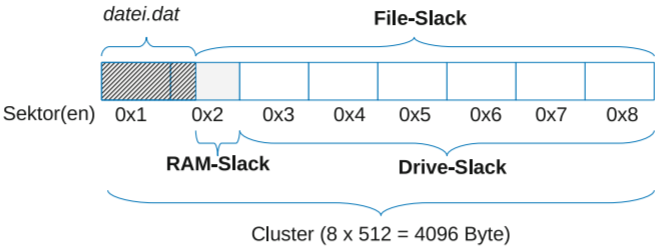
\includegraphics[width=0.55\textwidth]{bilder/File-Slack.PNG}
    		\caption{Zusammensetzung des File-Slacks innerhalb eines Clusters \cite[S. 133]{texbook02}}
		    \label{fig:fileslack}
	    \end{figure}
	    
        Updates sollen nur auf Empfehlung des Response-Team installiert werden \cite[vgl. S. 87]{texbook01}. Diese nicht sofort zu installieren, hat den Vorteil herauszufinden, welche Sicherheitslücke zum Sicherheitsvorfall geführt hat. Daher ist es sinnvoll, diese Lücke zumindest für einen kurzen Zeitraum offen zulassen. Das ist im Einzelfall abzuwägen, weil dadurch möglicherweise zusätzlicher Schaden entstehen kann. Genauso soll Software installiert oder deinstalliert werden, wenn das Response-Team es empfehlt. Da Beweise vernichtet werden können bei unüberlegtem installieren oder deinstallieren von Software. Forensik-Werkzeuge sollen jedoch nicht erst noch auf das kompromittierte System installiert werden. 
        
	    \subsubsection{Live-Sicherung - flüchtige Daten}
	    Flüchtige Daten sind nur temporär vorhanden wie Prozessregister und Datenpakete oder bis zum Ausschalten des Systems wie der RAM-Inhalt. In der Live-Sicherung wird daher versucht, die flüchtigen Daten in möglich kurzer Zeit am laufenden System zu sichern, ohne den Zustand des Systems zu ändern \cite[vgl. S. 119]{texbook02}. Dieses Vorgehen ist von Vorteil, wenn auf dem kompromittierten System kritische Anwendungen laufen und diese nicht durch ein Herunterfahren unterbrochen werden sollen. Die Live-Sicherung hat in den letzten Jahren an Relevanz gewonnen. Da die Repräsentation der Daten im System so nah wie möglich dem zum Zeitpunkt des Sicherheitsvorfalls entsprechen. Sowie sensible Informationen gesammelt werden können, die nach dem Ausschalten des Systems nicht mehr vorhanden sind. Je schneller die Daten gesichert worden, desto akkurater sind die gesammelten Ergebnisse. Ein identisches Abbild des Speichers zum Zeitpunkt des Sicherheitsvorfalls ist nachträglich unmöglich zu rekonstruieren \cite[vgl. S. 113]{texbook04}. Der große Nachteil der Live-Sicherung ist die Gefahr, bedeutsame Daten zu vernichten oder zu ändern durch unüberlegte Aktionen wie bereits in vorherigen Abschnitten beschrieben.

	    Die Daten sollen in einer RAM-Disk, auf eine Diskette oder über das Netz geschrieben werden. Um die Daten schnell zu sammeln, eignet sich die Verwendung von Skripten oder Batch-Dateien. Die zu sammelnden relevanten flüchtigen Daten sind das Systemdatum und die aktuelle Uhrzeit, sodass bearbeitete Zeitstempel ersichtlich werden und alle ausgeführten Befehle einen Startzeitpunkt zugeordnet werden können. Die Liste der laufenden Prozesse und dessen Metadaten, um eventuell schädliche Prozesse zu entdecken und genauer zu analysieren. Der komplette Inhalt des Hauptspeichers soll im Prozesskontext gesichert werden. Um die Auswertung zu erleichtern, sollte der Hauptspeicher eines zugeordneten Prozesses separat erfasst werden. Eine Liste der offenen Ports und Anwendungen, die auf offene Ports lauschen sollte dokumentiert werden. Es lässt sich daraus erkennen, ob Verbindungen gerade aufgebaut oder abgebaut werden. Werden beispielsweise sehr viele Verbindungsaufbauanfragen gefunden, kann davon ausgegangen werden, dass auf dem System ein Distributed Denial of Service (DDoS) Angriff oder ein Portscan ausgeführt wird \cite[vgl. S. 90]{texbook01}.
	    
	    \subsubsection{Post-mortem-Sicherung - persistente Daten}
	    In der Post-mortem-Sicherung werden die Daten im ausgeschalteten Zustand vom System gesichert \cite[vgl. S. 30]{texbook03}. Hierbei handelt es sich um persistente Daten in Datenträgern. Der Standardverfahren bei der Sicherstellung ist die forensische Duplikation. Dieser ist eine bitweise Kopie des Speicherabbilds eines Datenträgers, unabhängig von logischen Laufwerkzuordnungen. Der Datenträger wird aus dem kompromittierten System entfernt und an das Analysesystem der Ermittelnden angeschlossen und übertragen. Um ein versehentliches Überschreiben des Datenträgers zu verhindern, werden Writeblocker verwendet. Diese Geräte blockieren physisch den Schreibzugriff auf den zu sichernden Datenträger. Dieser ist auf dem Analysesystem weiterhin sichtbar, jedoch ist das Schreiben nicht möglich. Dritte können bei der juristischen Aufarbeitung nicht vorwerfen, unsauber gearbeitet zu haben, aufgrund versehentlichen Überschreibens. In \autoref{fig:Writeblocker} ist ein mobiler Writeblocker dargestellt, der zwischen das Analysesystem und dem Datenträger positioniert wird. Zusätzlich gibt es stationäre Writeblocker, die in dem Analysesystem eingebaut sind, welche häufig höhere Geschwindigkeiten erzielen. Bei der Erstellung einer forensischen Duplikation ist zu beachten, dass es auf dem Datenträger einige schwer zugreifbare Bereiche gibt, die Daten verstecken können. Deshalb soll das Verfahren für die Duplikation in der Lage sein, diese schwer zugreifbaren Bereiche zu identifizieren und zu sichern. Beispiele für schwer zugreifbare Bereiche sind der Host Protected Area (HPA) oder der Device Configuration Overlay (DCO) \cite[vgl. S. 26]{BSI-leitfaden2011}.
        \begin{figure}[h] 
    		\centering %mittig zentriert
    		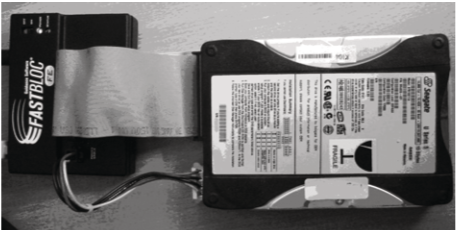
\includegraphics[width=0.485\textwidth]{bilder/Writeblocker.PNG}
    		\caption{Sicherung eines Datenträgers mit Hilfe eines Writeblockers \cite[S. 92]{texbook01}}
    	    \label{fig:Writeblocker}
	    \end{figure}
	    
	    Die Untersuchung eines Datenträgerabbilds mittels forensischer Duplikation bietet viele Vorteile. Im Gegensatz zur Sicherstellung von flüchtigen Daten in der Live-Sicherung, sind diese gegen Rootkits resistent \cite[vgl. S. 70]{BSI_leitfaden} und Ermittelnde können nicht regelmäßig in Gefahr laufen, Beweise zu vernichten. Das Duplikat kann beliebig oft kopiert werden und die Gefahr von Datenverlust oder Datenmodifikation besteht nicht, da Prüfsummen verwendet werden können. Die Kopien können an mehrere Ermittelnde verteilt werden und parallel zeitaufwendige Analysen durchführen. In der Zeit kann das kompromittierte System wiederhergestellt werden \cite[vgl. S. 92]{texbook01}.
	    
	    Zahlreiche Software- und Hardware-Werkzeuge stehen Ermittelnde bei der Erstellung forensischer Duplikationen zur Verfügung. Hardwarelösungen bieten häufig eine höhere Geschwindigkeit beim Duplizieren, womit die Sicherung von mehreren großen Datenträgern erleichtert wird. Für die korrekte Auswahl der Werkzeuge müssen wesentliche Anforderungen erfüllt sein. Die Datenübertragung muss bitweise erfolgen. Lesefehler müssen verlässlich abgefangen werden können. Bei mehrmaligen Leseversuchen fehlerhafter Sektoren müssen die markiert und mit Platzhalter versehen werden können. Der Zugriff muss lesend erfolgen, es dürfen keine Änderung an dem zu sichernden Datenträger vorgenommen werden. Die Anwendung muss reproduzierbar sein, damit Dritte bei den gleichen Aktionen die gleichen Ergebnisse erzielen. Die Integrität des Datenträgerabbilds muss durch Prüfsummen festgestellt werden, sodass diese vor unbemerkten Änderungen zuverlässig erkannt werden. Zu beachten ist, dass einige Hersteller angefangen haben, nicht das komplette Datenträgerabbild zur Verfügung zu stellen. Stattdessen extrahieren sie relevante Informationen im Vorfeld. Das bietet eine schnellere Duplikation und erspart einige Zwischenschritte. Andererseits müssen die Ermittelnden im Voraus entscheiden, welche Daten sie analysieren möchten. Die Komprimierung der Daten kann sich nachteilig auf die Ermittlung auswirken, weshalb eine vollständige Duplikation zu bevorzugen ist \cite[vgl. S. 93-94]{texbook01}.

%-----------------------------------------------------------------------------
\section {Juristische Beweisführung DL}
Die Grundlage für eine erfolgreiche Identifizierung möglicher Tatverdächtiger ist die Erhebung von Beweismitteln und deren rechtssichere Behandlung. Bei den häufigsten Spuren handelt es sich um digitale Spuren, die bei unsachgemäßer Behandlung ihren Beweiswert verlieren und möglicherweise sogar völlig unbrauchbar werden. 

Sachbeweise sind verfahrensrechtliche Beweismittel, die Strafverfolgungsbehörden und Gerichte zum Nachweis von Straftaten oder strafbaren Handlungen dienen. Zu diesen gehören z. B. Datenträger, bestimmte Logdateien oder Gutachten \cite[vgl. 78]{texbook01}.
Die Beweiskraft wird erst durch die Person deutlich, die die Beweise sammelt und die Beweise in den strafrechtlichen Zusammenhang stellt und interpretiert. Daher sind Sachbeweise eng mit persönlichen Beweisen verbunden. 
Die Integrität und Glaubwürdigkeit derjenigen, die Beweise erbringen, sind wesentliche Elemente der Bedeutung von Beweismitteln.
Hier ist klar, dass Beweismittel an Glaubwürdigkeit verlieren können, sobald sie durch eine Person verzerrt wurden oder auch nicht belegte Behauptungen oder Interpretationen zum Beweis aufstellen \cite[vgl. S. 79]{texbook01}. 
Sämtliche sachlichen Beschreibungen, angewandten Verfahren und Bedeutungsinterpretationen, beispielsweise die der Täter und Täterinnen werden sorgfältig durch die Richter und Richterinnen geprüft. %----------
Der Beweis selbst, aber auch die Person, die ihn erbracht hat, sind von gleicher Bedeutung für das Verfahren. Denn abhängig von der Entscheidung der Richter und Richterinnen über die Glaubwürdigkeit der Person, die den Beweis geliefert hat, wird der Gebrauchswert des Beweises im Entscheidungsprozess ermittelt \cite[vgl. S. 98]{texbook03}.

Eine sorgfältige Dokumentation der Aktivitäten der Beweiserhebung unterstützt die Glaubwürdigkeit der Beweise und dient als Nachweis genauer Untersuchungen.
Zugunsten des Urteils muss strikt zwischen festgestellten Tatsachen vor Gericht und persönlicher Wertung getrennt werden.
Es ist daher immer zu beachten, dass es um Zahlen, Daten und Fakten gehen muss.

Hierbei können Probleme auftreten, wenn den Beteiligten aufgrund unterschiedlicher Wissensstände die technischen Hintergründe des Falls nicht bewusst sind.
Weshalb es umso notwendiger ist, Sachverhalte verständlich und nachvollziehbar darzustellen.
Interpretationen müssen dementsprechend auch dargestellt werden.
Vor Gericht besteht oft der Grund zur Verwechslung von Tatsachen und Annahmen und diese gilt es zu differenzieren. 

    \subsection{Datenschutz}
    Bei computerforensischen Ermittlungen ist die Erhebung, Nutzung und Verarbeitung großer Datenmengen mit personenbezogenen Informationen aus allen Lebensbereichen nicht auszuschließen. Trotz umfangreicher Auswertung von Datenträgern und Postfächern besteht daher eine der zentralen Herausforderungen der Computer-Forensik darin, die individuellen Rechte der Betroffenen angemessen zu wahren \cite[vgl. S. 72]{texbook03}.
    Beim Auswerten dieser Daten kommen unumgänglich Fragen bezüglich des Datenschutzes auf.
    Grundlage des Datenschutzes ist das Recht auf informationelle Selbstbestimmung, das Bundesdatenschutzgesetz a.F. § 3a Datenvermeidung und Datensparsamkeit legt die Grundprinzipien des Datenschutzes fest:
    \begin{quote}
        \glqq
        Die Erhebung, Verarbeitung und Nutzung personenbezogener Daten und die Auswahl und Gestaltung von Datenverarbeitungssystemen sind an dem Ziel auszurichten, so wenig personenbezogene Daten wie möglich zu erheben, zu verarbeiten oder zu nutzen. Insbesondere sind personenbezogene Daten zu anonymisieren oder zu pseudonymisieren, soweit dies nach dem Verwendungszweck möglich ist und keinen im Verhältnis zu dem angestrebten Schutzzweck unverhältnismäßigen Aufwand erfordert.
        \grqq
        \cite[S. 1]{bg3a}
    \end{quote}
    Gemäß § 31 BDSG sind Daten ausschließlich zur Datenschutzkontrolle, der Datensicherung oder zur Sicherstellung eines ordnungsgemäßen Betriebes der Datenverarbeitungsanlage speicherbar \cite[vgl. S. 1]{bg31}. Diese Daten umfassen Daten zur Zugangskontrolle, Netzwerk- und Verkehrsinformationen wie IP-Adressen oder Anrufer-IDs und Protokolldaten wie Anmelde- und Abmeldezeiten von Benutzer und Benutzerinnen.
    
    Bei der Durchführung von Untersuchungen gilt nach wie vor der Datenschutz und kann grundsätzlich nicht außer Kraft gesetzt werden. Das Gesetz gibt Behörden jedoch das Recht, Informationen zu sammeln, auf die sie aufgrund des Datenschutzes eigentlich keinen Zugriff haben. Datenschutz sollte in diesem Zusammenhang nicht Tatenschutz/Täterschutz sein. Der Grundsatz des Datenschutzrechts lautet daher, dass Datenübermittlungen erfolgen dürfen, weil die einschlägigen Strafverfahrensgesetze die zuständigen Behörden dazu ermächtigen \cite[vgl. S. 83]{texbook01}.
    Die Auskunftspflicht über die Daten wird dadurch berührt, dass der Dateninhaber oder die Dateninhaberin die zu bezeugende Person ist. Wenn der Eigentümer der Daten daher vor Gericht als Zeuge oder Zeugin eingeladen wird, muss er Auskunft über diese Daten geben.
    
    \subsection{Beweisspuren sichern}
    Für die Ermittlung lassen sich auf IT-Systemen einige interessante sensible Datenarten finden, die den Ermittlungen von Vorteil sein können (siehe \nameref{DigitaleSpurensicherung}).\\
    Es gibt flüchtige Daten wie z.B. Inhalt von Cache und Hauptspeicher, Netzwerkverbindungsstatus und laufende Prozesse.
    Dem Gegenüber existieren auf der Festplatte persistente abgespeicherte Daten, deren Zustand und Zeitstempel sich aber bei Zugriff ändert. Semipersistente Daten sind temporäre Informationen, die sich auf der Festplatte befinden, auf die nur zu bestimmten Zeiten zugegriffen werden kann, während beispielsweise eine Anwendung ausgeführt wird.
    
    Zur Beweissicherung sollten unbedingt sterile Datenträger verwendet werden. Diese müssen virenfrei sein und idealerweise sollten Medien vor der Verwendung zuverlässig formatiert und von allen Spuren früherer Daten gereinigt werden. Dies sollte vor der Verwendung überprüft werden \cite[vgl. S. 82]{texbook01}. 
    Der Vollständigkeit halber sollten Werkzeuge und Methoden zur Beweisfindung und -sicherung vorab getestet werden. Sinnvollerweise, sollte hier zu allgemein anerkannten Verfahren und Instrumenten gegriffen werden.

    \subsection{Bewertung der Beweisspuren} 
    In der Analysephase (siehe \nameref{SAP}) werden die in der Sicherungsphase erfassten Daten darauf untersucht, ob sie Beweisspuren zur Aufklärung des relevanten Sachverhalts enthalten. Grundsätzlich lassen sich drei Gruppen von Beweisspuren unterscheiden.  Beweisspuren, die eine bestimmte Theorie stützen. Sowie Beweisspuren, die hinführend zu einer bestimmten Theorie führen. Abschließend Beweisspuren, die keine bestimmte Theorie stützen oder widerlegen, sondern nur aufzeigen, dass das System verändert wurde, um Informationen oder Spuren zu verbergen \cite[vgl. S. 83]{texbook01}. Bei der Auswertung der Ergebnisse einer Analyse sollte immer klar sein, zu welcher Gruppe die gefundenen Informationen gehören und was sie letztendlich aussagen.
    
	\subsection{Durchgeführte Aktionen dokumentieren}
    Alle während einer Untersuchung durchgeführten Maßnahmen müssen dokumentiert werden. Sinnvoll ist, vorab ein eigenes Dokumentenformat zu definieren und entsprechende Formulare bereitzuhalten. Exemplarisch ist in \autoref{fig:Dokumentation} solch ein Dokumentenformat abgebildet. Auch hier ist es wichtig, dass Dritte die Dokumentation nachvollziehen und unbefugte Änderungen verhindern können. Das Dokument kann unter Umständen letztendlich die Glaubwürdigkeit einer Untersuchung untermauern, die zu belastenden Beweisen geführt hat.    
    
    \begin{figure}[h] 
    	\centering
    	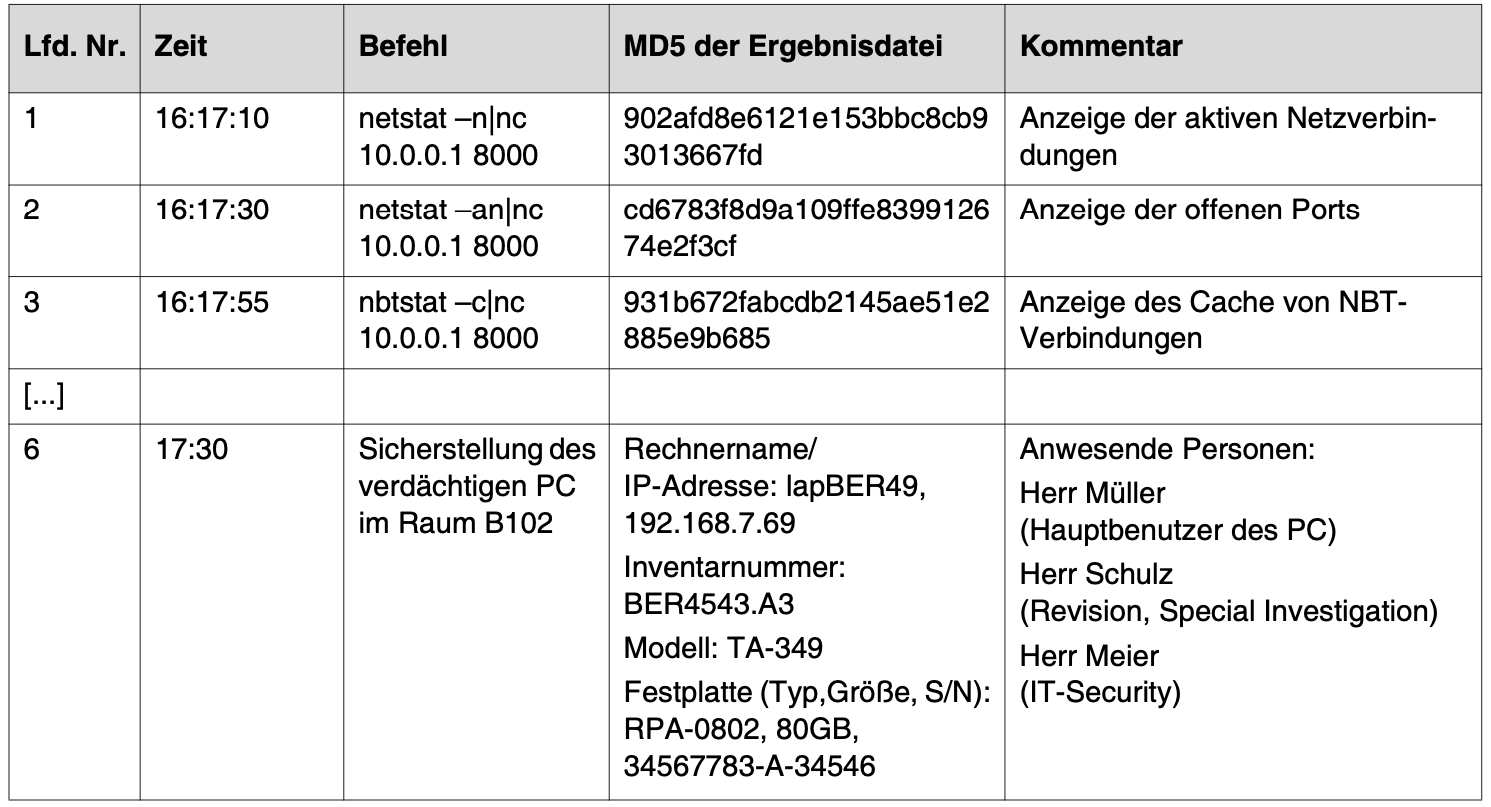
\includegraphics[width=0.8\textwidth]{bilder/dokumentation_von_aktionen.png} 
    	\caption{Beispiel einer Dokumentation der durchgeführten Aktion \cite[S. 84]{texbook01}}
    	\label{fig:Dokumentation}
    \end{figure}
	Neben den allgemeinen Untersuchungsgründen sollte für jede einzelne Maßnahme dokumentiert werden, weshalb die einzelnen Vorgehensschritte durchgeführt wurden und welche Erkenntnisse daraus zu erwarten sind. In jedem Fall sollten verdächtige Dateien zur späteren Analyse kopiert werden. Außerdem sollten Screenshots ausgiebig in Verwendung kommen, um die erzielten Ergebnisse besser auswerten zu können, sollte das verwendete Prüfungstool mit seiner Versionsnummer erfasst werden.
    
    \subsection{Beweise dokumentieren}
    Bei gesicherten Beweismitteln wie Festplatten, Notebooks oder Dokumente muss eine lückenlose Beweiskette gewährleistet sein. Es sollte jederzeit nachvollziehbar sein, welche Person zu welchem Zeitpunkt wie auf diese Nachweise Zugriff hatte. Wie in \autoref{fig:Beweiszettels} sollen alle gefundenen Beweise auf einem Beweiszettel vermerkt werden.
    \begin{figure}[h]
        \centering
        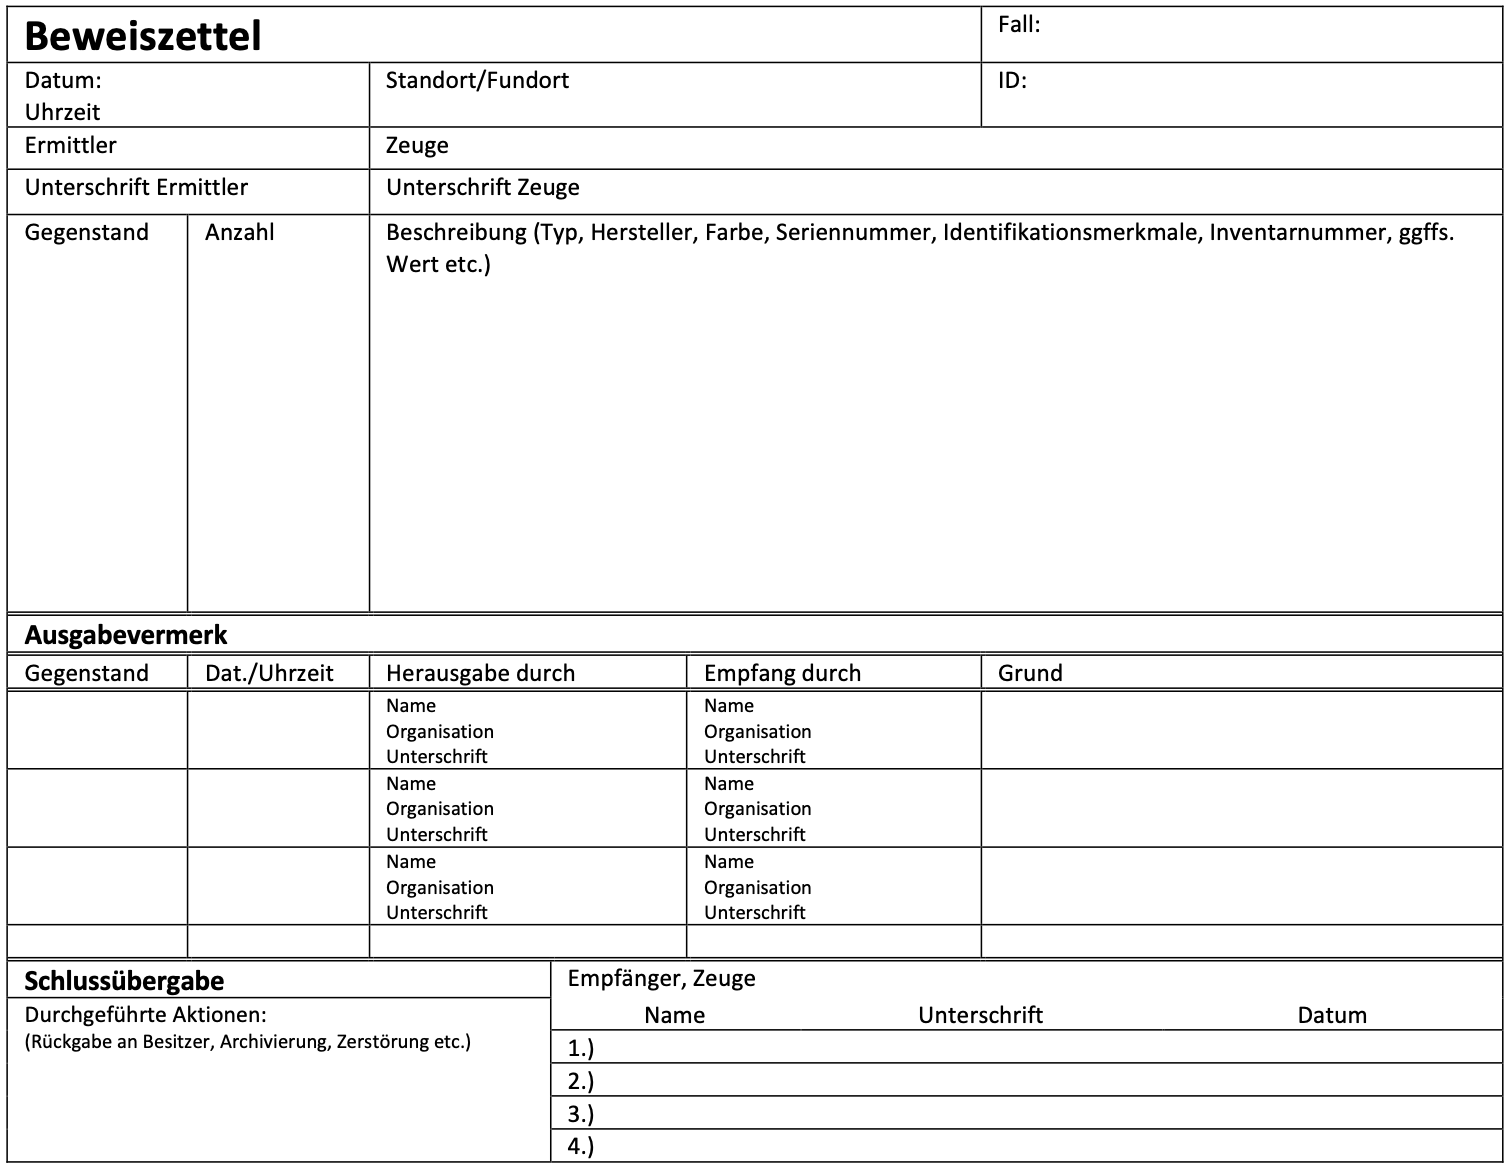
\includegraphics[width=0.9\textwidth]{bilder/Beweiszettels.png} 
        \caption{Beispiel eines Beweiszettels}
        \label{fig:Beweiszettels}
    \end{figure}
    
    Aufgefundene Beweise sollten so dokumentiert werden, dass bei späteren rechtlichen Ermittlungen kein Zweifel über Herkunft, Besitztum und Integrität aufkommen kann \cite[vgl. S. 85]{texbook01}. 
    Aus diesem Grund ist es ratsam, für jeden gefundenen oder beschlagnahmten Gegenstand einen Beweiszettel anzulegen und Eigentümer des Objekts, falls er ermittelt werden kann, zu notieren. Zusätzlich ist diesem Nachweisblatt eine ausführliche Objektbeschreibung beizufügen. Insbesondere wenn mehr als eine Person oder Organisation an der Untersuchung beteiligt sind, sollte dokumentiert werden, wer zu welchem Zeitpunkt aus welchem Grund Zugriff auf die Beweise hatte.

    Neben dem Beweismittel selbst ist oft besonders wichtig, wo es gefunden wird. Zu diesem Zweck sollte auch festgehalten sein, wo und unter welchen Umständen verdächtige Gegenstände gefunden wurden. Auch hier hängt der Aufwand, Beweise zu sammeln, von der Art des Sicherheitsvorfalls und seinem Umfang ab.

\section {Erste Schritte an einem System für die Sicherstellung DL} 
Unabhängig welches Betriebssystem verwendet wird, sind beim Schutz verdächtiger Client-PCs einige allgemeine Schritte zu beachten. Bei Serversystemen kann es zu abweichenden Handlungen kommen, weshalb nötige Vorüberlegungen zu treffen sind, um im Falle einer eigenverantwortlichen Beschlagnahme angemessen vorzugehen.

	\subsection{Fall 1: System läuft nicht}	 
	Im Fall, dass das System nicht läuft, sollten folgende Vorkehrungen befolgt werden:  \\ 
	Zunächst ist es wichtig alle Verbindungen zu fremden Personen vom System und der Stromversorgung zu entfernen. Es sind Umgebungsfotos und ggf. Skizzen vom Standort der Systeme und Peripherie-Geräte anzufertigen. Arbeiten noch laufende Prozesse  wie \\z. B. Druckjobs, ist es ratsam diese zu Ende laufen zu lassen. Das System darf auf keinen Fall eingeschaltet werden, dabei ist darauf zu achten, dass sich das System auch automatisch nach dem Aufklappen bei Laptops einschalten kann. Sicherzustellen ist auch, dass das System tatsächlich heruntergefahren ist. Bei Laptops kann der Akku entfernt werden, um sicherzustellen, dass der Energiemodus nicht aktiviert und möglicherweise der Zeitstempel geändert wird. Andernfalls sollten die Netzkabel von den Geräten abgezogen werden. Ist zusätzlich die WakeOnLan-Funktion mit eingebaut, sollte auch das Netzkabel entfernt werden. Für  alle beschlagnahmten Gegenstände gilt es, diese eindeutig zu kennzeichnen. Bei der Suche nach Hinweisen sollte auch um den Bereich nach Notizen und Papieraufzeichnungen geachtet werden \cite[vgl. S. 96]{texbook01}. Wenn möglich, ist es hierbei von großem Vorteil den Anwender nach Systembesonderheiten, Passwörtern oder anderen spezifischen Konfigurationen des Systems gründlich auszufragen, bei dessen Antworten es gilt diese präzise aufzuzeichnen, allerdings auch kritisch zu hinterfragen. Beim gesamten Vorgehen ist es unabdingbar eine vollständige Dokumentation aller Aktivitäten, durch die beschlagnahmte Hardware, zu führen.

	\subsection{Fall 2: System läuft}	 
	Liegt der Fall vor, dass das System läuft, sollte folgendermaßen vorgegangen werden:  \\ 
	Wie im 1. Fall muss das System von jeglichen Verbindungen zu fremden Personen isoliert werden, Umgebungsfotos und ggf. Skizzen angefertigt werden und für genauere Aktivitäten und Angaben des Systems, der Anwender ausgefragt werden. Zu untersuchen gilt nun im eingeschalteten Zustand ebenfalls sämtlicher Bildschirminhalt. Dieser sollte mit einer Digitalkamera oder einem ähnlichen Gerät erfasst werden. Dabei ist es wichtig, Peripheriegeräte nicht zu berühren, um eine Änderung des Zeitstempels zu vermeiden \cite[vgl. S. 97]{texbook01}. Muss unter Umständen etwas geändert werden, sollte dies notiert und die Erlaubnis des Ermittlungsleiters eingeholt werden. Wichtig ist, alle Aktivitäten zeitgenau aufzuzeichnen \cite[vgl. S. 53]{BSI_leitfaden}.

	\subsection{Entscheidungsprozesse}
	Sicherheitsvorfälle unterscheiden sich von Fall zu Fall und müssen individuell betrachtet werden. Dabei können für jeden Vorfall auch besondere Entscheidungen erforderlich sein. Eine Weiterleitung an ein beliebig höheres Glied der digitalen Rettungskette ist notwendig, wenn die ausgesprochenen Handlungsempfehlungen die Problematik nicht lösen konnten oder keine eindeutige Bestimmung des Sachverhaltes möglich ist.
	In Anlehnung der Empfehlungen des Bundesamtes für Sicherheit in der Informationstechnik kann das in \autoref{fig:Entscheidungsmatrix} folgende Ablaufdiagramm als Basis dienen \cite[vgl. S. 53]{BSI_leitfaden}.

	\begin{figure}[h] 
		\centering
		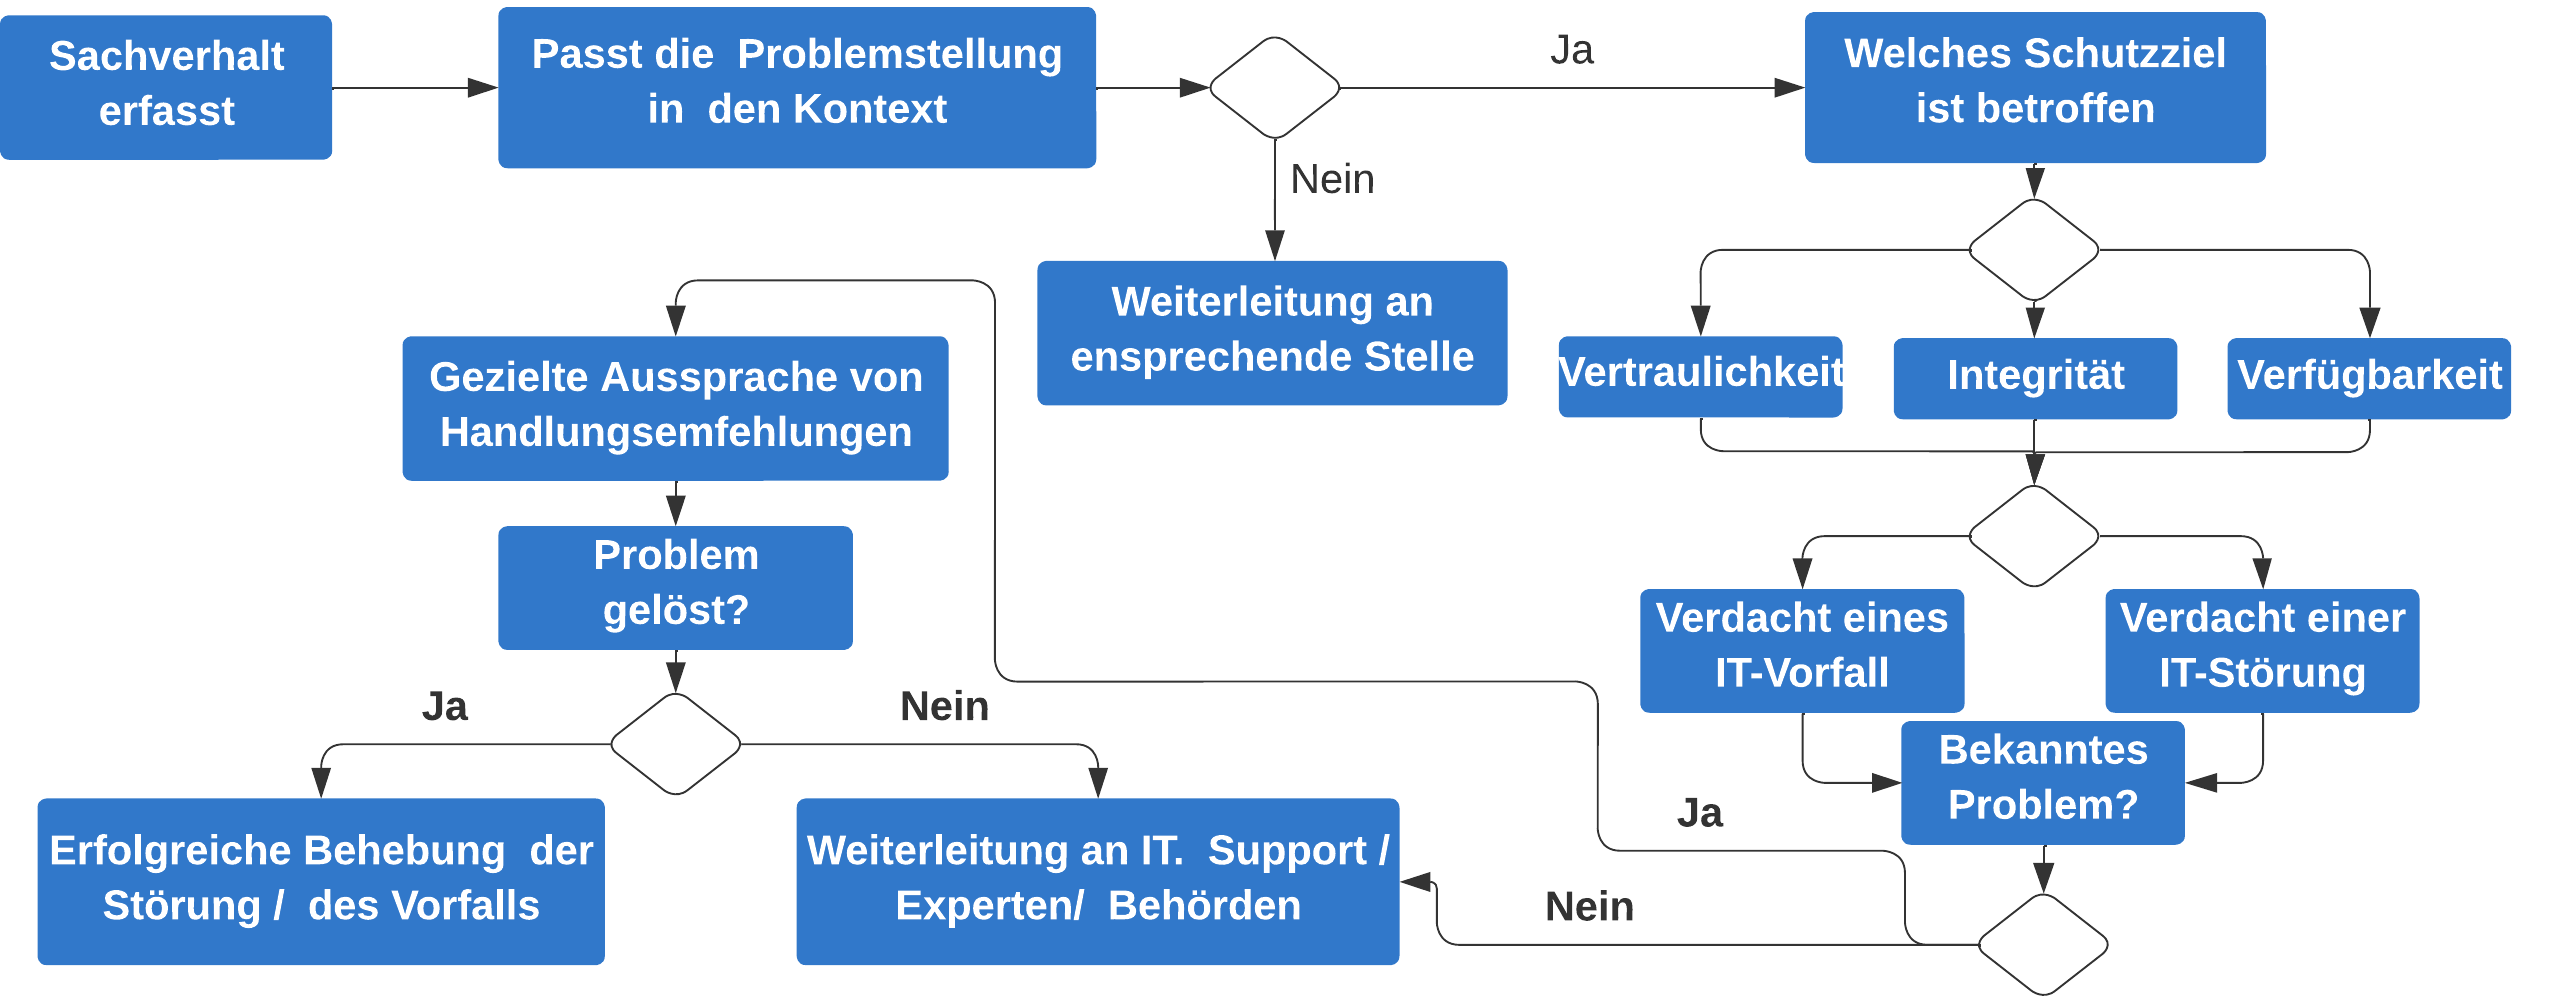
\includegraphics[width=1.0\textwidth]{bilder/Entscheidungsmatrix2.png} 
		\caption{Entscheidungsmatrix}
		\label{fig:Entscheidungsmatrix}
	\end{figure}

    Zuerst muss der Sachverhalt erfasst werden, dann wird überprüft, ob die Problemstellung in den Kontext passt, ist dies nicht der Fall sollte eine Weiterleitung an die entsprechende Stelle erfolgen. Ansonsten ist zu prüfen, welche Schutzziele betroffen sind und es muss unterschieden werden, ob es sich um einen IT-Vorfall oder eine IT-Störung handelt. Ist es ein unbekanntes Problem, muss es dem IT-Support weitergeleitet werden. Wenn dem nicht so ist, sollte man die vorgeschlagene Vorgehensweise befolgen. Wenn dies das Problem nicht löst, sollten Sie sich nun an den IT-Support wenden.

\section {Schluss DL und SAK}
Die Computer-Forensik hat in den letzten Jahren durch zunehmenden Angriffe auf Systeme sowie die leichtere Verfügbarkeit und Verwendung von Werkzeugen im Internet für Angriffe sehr an Bedeutung erlangt. Dessen Bedeutung wird sich in den nächsten Jahren durch die zunehmende Digitalisierung in vielen Lebensbereichen und kritischer Infrastruktur weiter festigen.  
Bei der Ermittlung sind grundsätzliche Aspekte zu berücksichtigen. Die eingesetzten Methoden und Werkzeuge sollten von Experten anerkannt, robust und die Ergebnisse reproduzierbar sein. Damit die gesammelten Beweise rechtsverbindlich sind, muss deren Integrität gewährleistet und jeder Schritt detailliert dokumentiert werden.

Nach dem SAP-Modell gliedert sich die Ermittlung in drei große Phasen. Die erste Phase \textit{Secure} befasst sich mit der sorgfältigen Erfassung aller Daten. Damit die gesammelten Daten ihre juristische Belastbarkeit nicht verlieren, werden sie nach dem Vier-Augen-Prinzip erhoben und ihre Integrität durch Prüfsummen sichergestellt. In der zweiten Phase \textit{Analyse} werden die Ergebnisse ausgewertet und kritisch hinterfragt. Abschließend werden in der \textit{Present} Phase die ausgearbeiteten Ergebnisse zielgruppenorientiert präsentiert. 
Eine sinnvolle Erweiterung des SAP-Modells ist eine zusätzliche Vorbereitungsphase zu Beginn, in der die Rahmenbedingungen der Ermittlung festgehalten werden. Die Ziele und der Zweck der Ermittlung sollen klar ersichtlich werden und die zur Verfügung stehenden Ressourcen feststehen.

Zentral ist die Sicherung von digitalen Spuren, die zwangsläufig bei einem Angriff entstehen. Es ist einem Angreifer unmöglich, alle Spuren zu vernichten. Der erste Schritt bei der Spurensicherung ist, die aktuelle Uhrzeit zu dokumentieren, um veränderte Zeitstempel nachvollziehen zu können. Alle ausgeführten Befehle und Maßnahmen müssen dokumentiert werden. Hilfreich ist dabei ein einheitliches Dokumentenformat, indem der Zweck und die Erwartungen der einzelnen Schritte aufgezeichnet werden. Laufende Befehle dürfen nicht beendet und die Ausgaben von Befehlen soll auf ein anderes Dateisystem geschrieben werden, um Beweise nicht zu vernichten.
Es gibt zwei Sicherungsvarianten, die Live-Sicherung und die Post-mortem-Sicherung. Die Live-Sicherung eignet sich zum Sichern flüchtiger Daten, bei denen das System während der Untersuchung und Datensammlung weiter betrieben wird. Es besteht die Gefahr, dass während der Datensammlung Beweise vernichtet werden können. Daher ist die Live-Sicherung nur in besonderen Fällen sinnvoll, beispielsweise wenn kritische Anwendungen auf dem System laufen und dieser nicht heruntergefahren werden soll. In der Post-mortem-Sicherung wird eine forensische Duplikation des Datenträgers vom ausgeschalteten System erstellt. Dies hat den großen Vorteil, dass Kopien beliebig oft angefertigt werden können und das Risiko der Beweisvernichtung minimiert wird. Ebenfalls können durch die Kopien mehrere zeitaufwändige Analysen parallel durchgeführt werden. Weshalb die Post-mortem-Sicherung in den meisten Fällen der Live-Sicherung vorzuziehen ist.

Schwierigkeiten bereiten die gesetzlichen Rahmenbedingungen zum Datenschutz, welche private Ermittlungen stark einschränken und die Erfolgsaussichten minimieren können. 
Die größte Herausforderung bei jeder forensischen Ermittlung besteht darin, all die gesammelten Beweise in einen kausalen und zeitlichen Zusammenhang zu stellen und daraus angemessene Schlussfolgerungen zu ziehen.

% Literatur
\pagebreak
\printbibliography
\listoffigures

\end{document}